\documentclass[crop,tikz]{standalone}

\usepackage{pgfplots}
\colorlet{green}{black!40!green}

\tikzset{>=latex}

\pgfplotsset{
  every non boxed x axis/.append style={
    axis line style={-latex}
  },
  every non boxed y axis/.append style={
    axis line style={-latex}
  },
  inverted/.style = {
    every axis legend/.append style={
      draw=white,
      fill=black,
      text=white
    }
  }
}

\begin{document}
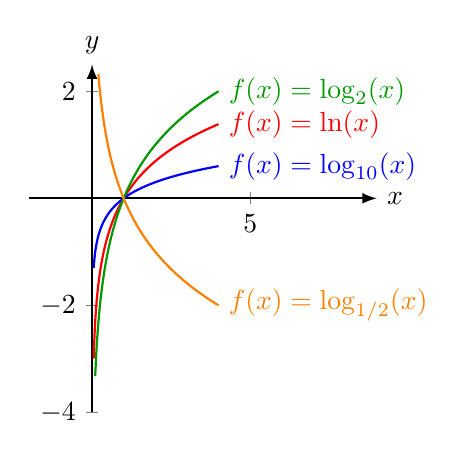
\begin{tikzpicture}
\begin{axis}[
  thick,
  width=6cm,
  height=6cm,
  domain=0.05:4,
  samples=100,
  smooth,
  axis y line=middle,
  axis x line=middle,
  xlabel={$x$},
  ylabel={$y$},
  xlabel style={right},
  ylabel style={above},
  xmin=-2, xmax=9,
  ymin=-4, ymax=2.5,
  clip=false
  ]
  \addplot[red] { ln(x) } node[right] {$f(x)=\ln(x)$};
  \addplot[blue] { log10(x) } node[right] {$f(x)=\log_{10}(x)$};
  \addplot[green,domain=0.1:4] { log2(x) } node[right] {$f(x)=\log_{2}(x)$};
  \addplot[orange,domain=0.2:4] { -log2(x) } node[right] {$f(x)=\log_{1/2}(x)$};
\end{axis}
\end{tikzpicture}
\end{document}
